\chapter{Methodology}

\begin{figure}[H]
	\centering
	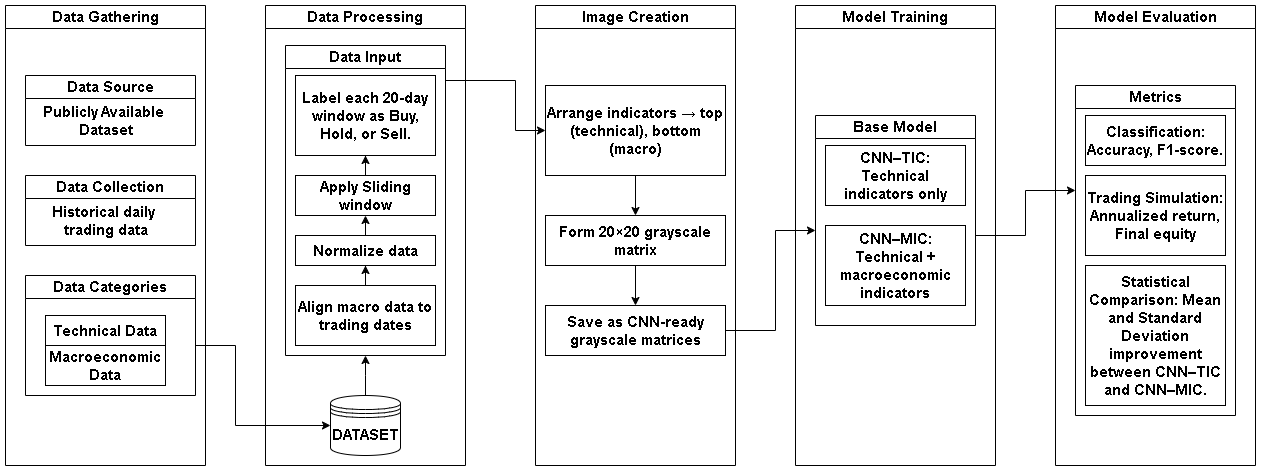
\includegraphics[width=1\textwidth]{../figures/Proposed Framework.png}
	\caption{Proposed Approach}
	\label{Figure 3: Proposed Framework}
\end{figure}


Figure~\ref{Figure 3: Proposed Framework} outlines the five stages of our methodology: (1)Data Gathering, (2)Data Processing, (3)Image Creation, (4)Model Training, and (5)Model Evaluation. The flow is centered on building an image representation of the combined technical and macroeconomic indicators using 20 lookback windows $L \in \{6,\ldots,25\}$ for each trading day.


\subsection{Data Gathering}
\label{subsec:data-gathering}

Open, High, Low, Close, and Volume (OHLCV) data from 2012 to August 2025 were collected for the selected PSE stocks and cryptocurrency assets. These values served as the basis for computing the technical indicators used in the image creation stage. In addition, five macroeconomic series were collected to represent the broader market environment: Reverse Repurchase (RRP), purchasing power of the peso (PPP), inflation rate, gold, and crude oil.

\subsection{Data Processing} \label{subsec:data-processing}
This stage ensures proper \emph{time alignment}, \emph{normalization}, and \emph{labeling} before creating images. We process two groups of variables in parallel, the technical indicators and the macroeconomic indicators, and merge them in \emph{Image Creation}.

\subsubsection*{(A) Processing of the technical indicators}

Following the technical indicator set used in CNN--TIC, the following 15 technical indicators are computed using the \texttt{ta} Python library~\cite{ta-bukosabino}: RSI, Williams~\%R, SMA, EMA, WMA, HMA, TEMA, CCI, CMO, MACD, PPO, ROC, CMFI, DMI, and PSI. These indicators are derived from OHLCV values and represent four main types of market information. First, trend indicators such as SMA, EMA, WMA, HMA, and TEMA summarize the direction of price movement by smoothing closing prices across a lookback window. Second, momentum indicators such as RSI, Williams~\%R, CMO, MACD, PPO, and ROC measure the speed, strength, or direction of price changes. Third, range-based indicators such as CCI, DMI, and PSI use high, low, and close values to describe trend strength, reversal behavior, or deviation from a typical price level. Finally, CMFI incorporates volume by measuring whether buying or selling pressure is supported by traded volume. These definitions follow common technical analysis formulations, while the actual computation in this study follows the implementation provided by the \texttt{ta} library~\cite{wilder1978new,murphy1999technical,achelis2001technical,ta-bukosabino}.

For each indicator $i$ and each lookback length $L \in \{6,7,\ldots,25\}$, we obtain the daily value
\[
x_{i,L,t} \;\; \text{for trading day } t.
\]
Here, $x_{i,L,t}$ denotes the value of technical indicator $i$ computed using lookback length $L$ for trading day $t$. Each lookback length produces one column in the technical image representation. Thus, one indicator generates 20 values per trading day, corresponding to window lengths from 6 to 25 days. Since there are 15 technical indicators, the technical-only representation contains $15 \times 20$ values before normalization and quantization.

For single-window indicators, $L$ sets the main computation window. For multi-parameter indicators such as MACD and PPO, $L$ controls the primary window according to the standard parameterization used by the library unless otherwise specified in the implementation. This step produces a structured technical feature matrix where rows correspond to indicators and columns correspond to lookback windows.
\subsubsection*{(B) Processing of the macroeconomic indicators}
Five macroeconomic indicators are aligned to the trading calendar with forward‑fill for non‑trading days: \textbf{RRP}, \textbf{PPP}, \textbf{inflation rate}, \textbf{gold}, and \textbf{crude oil}. To mirror the technical indicator format, we compute simple moving averages at the same set of lookbacks:
\[
\mathrm{SMA}_{m,L,t} = \frac{1}{L} \sum_{k=0}^{L-1} s_{m,t-k}, \qquad L \in \{6,\ldots,25\},
\]
where $s_{m,t}$ is the level of the macro series $m$ on day $t$.
\paragraph{Normalization and 8‑bit quantization.}
Each feature–lookback pair is first normalized with training‑only statistics, then quantized to unsigned 8‑bit:
\[
\tilde{v}_{r,L,t} = \operatorname{clip}\!\left(\frac{v_{r,L,t} - a_{r,L}}{b_{r,L} - a_{r,L} + \epsilon}, 0, 1\right),
\]
\[
\widehat{v}_{r,L,t} = \operatorname{round}\!\big(255 \cdot \tilde{v}_{r,L,t}\big) \in \{0,\ldots,255\},
\]
where $v_{r,L,t}$ is $x_{i,L,t}$ (technical) or $\mathrm{SMA}_{m,L,t}$ (macro); and $a_{r,L}, b_{r,L}$ are the minimum/maximum estimated \emph{on the training split only}. For training, images are loaded as float and rescaled by $1/255$ so inputs lie in $[0,1]$. Min–max scaling is used to preserve relative intensity patterns in the grayscale image, since CNN filters operate on spatial contrast, making consistent 0–255 scaling important.


\subsubsection*{(C) Label generation (\textit{Buy/Hold/Sell})}
The label for each trading day is generated using a fixed turning-point rule derived from previous CNN-based trading studies \cite{maratkhan2021deep}. 
A symmetric 11-day window consisting of five days before the current day, the current day, and five days after it is used. 
The purpose of this window is to determine whether the current price is a local minimum, local maximum, or not a turning point. 
It is important to clarify that the five future days in the 11-day window are used only for generating ground-truth labels during supervised training and evaluation. 
Future prices are not included as input features in CNN--TIC or CNN--MIC. 
In actual image creation and model prediction, the input image for trading day $t$ consists only of technical and macroeconomic indicators available up to day $t$. 
Therefore, the future window is only part of the supervised labeling process and is not part of the information received by the model during prediction.
Let $P_t$ be the adjusted close price on day $t$. 
Let $W_t = \{t-5,\ldots,t,\ldots,t+5\}$ be the 11-day labeling window centered on day $t$. 
The labeling rule is defined as
\begin{equation}
	y_t =
	\begin{cases}
		\textbf{Sell}, & \text{if } P_t = \max\limits_{\tau \in \mathcal{W}_t} P_\tau,\\[4pt]
		\textbf{Buy},  & \text{if } P_t = \min\limits_{\tau \in \mathcal{W}_t} P_\tau,\\[4pt]
		\textbf{Hold}, & \text{otherwise.}
	\end{cases}
	\label{eq:label}
\end{equation}
Algorithm 1 gives the exact implementation used in this study, including the handling of edge dates and ties, where non-unique extrema default to the Hold class. 
The generated labels were then used as the target classes during training, validation, and testing. 
The future portion of the 11-day window was not used to construct the CNN input images and was not available to the model during inference.

\begin{algorithm}[H]
	\caption{Turning point label generation (Buy, Hold, Sell)}
	\label{alg:labelgen-turningpoint}
	\begin{algorithmic}[1]
		\Procedure{LABELGEN\_TURNINGPOINT}{}
		\State $N = \text{length}(\text{close\_prices})$  \Comment{close\_prices\ = Daily close price series}
		\State $R \gets 5$ \Comment{11-day window, 5 days before and after}
		\For{$t = 0$ to $N - 1$}
		\State $start \gets \max(0, t - R)$
		\State $end \gets \min(N - 1, t + R)$
		\State \texttt{window} $\gets$ \texttt{close\_prices[start..end]}
		\State \texttt{center\_price} $\gets$ \texttt{close\_prices[t]}
		\State \texttt{max\_price} $\gets \max(\texttt{window})$
		\State \texttt{min\_price} $\gets \min(\texttt{window})$
		\State \texttt{max\_count} $\gets$ number of positions in \texttt{window} equal to \texttt{max\_price}
		\State \texttt{min\_count} $\gets$ number of positions in \texttt{window} equal to \texttt{min\_price}
		\If{\texttt{center\_price} = \texttt{max\_price} and \texttt{max\_count} = 1}
		\State \texttt{label\_text[t]} $\gets$ ``Sell''
		\State \texttt{label\_code[t]} $\gets -1$
		\ElsIf{\texttt{center\_price} = \texttt{min\_price} and \texttt{min\_count} = 1}
		\State \texttt{label\_text[t]} $\gets$ ``Buy''
		\State \texttt{label\_code[t]} $\gets 1$
		\Else
		\State \texttt{label\_text[t]} $\gets$ ``Hold''
		\State \texttt{label\_code[t]} $\gets 0$
		\EndIf
		\EndFor
		\State save table with columns: dates, close\_prices, label\_text, label\_code
		\State \Return \texttt{label\_code}
		\EndProcedure
	\end{algorithmic}
\end{algorithm}


\subsection{Image Creation} \label{subsec:image-creation}
We generate two types of grayscale images for each trading day: a $15 \times 20$ technical-only image and a $20 \times 20$ combined technical and macroeconomic image. Both follow the same lookback length, using 20 window lengths from $L = 6$ to $L = 25$.

The first representation is used by CNN--TIC. 
It has a size of $15 \times 20$ because it consists of 15 technical indicator rows and 20 lookback columns. 
The second representation is used by CNN--MIC. 
It keeps the same 15 technical rows and the same 20 lookback columns, but adds five macroeconomic rows. 
As a result, the image matrix expands from $15 \times 20$ to $20 \times 20$. 
The change is in the number of rows, not in the number of lookback windows.

\paragraph{Combined image construction.}
For the full representation, we construct a matrix $I \in \mathbb{Z}^{20 \times 20}_{[0,255]}$ with the following layout:
\begin{enumerate}
	\item \textbf{Rows.} Rows $1\text{–}15$ correspond to the technical indicators in a fixed order. Rows $16\text{–}20$ correspond to the macroeconomic series in the order \{RRP, Gold, Crude Oil, PPP, Inflation\}.
	\item \textbf{Columns.} Column $c \in \{1,\ldots,20\}$ corresponds to lookback $L = 5 + c$, spanning $L = 6,\ldots,25$.
	\item \textbf{Pixel assignment.} For technical row $i$ and column $c$, set $I_{i,c} = \widehat{x}_{i,L,t}$. For macro row $k$, set $I_{15+k,c} = \widehat{\mathrm{SMA}}_{k,L,t}$.
\end{enumerate}
In earlier studies such as CNN--TIC, the technical indicators are grouped into clusters based on their similarity, and these clusters are placed into predefined regions of the image \cite{maratkhan2021deep}. Clustering is used to reveal relationships among indicators and to guide the spatial arrangement of the image. In this study, we do not apply any clustering procedure. Instead, a fixed and consistent layout is used across all images. The fifteen technical rows correspond directly to fifteen indicators (RSI, WilliamsR, SMA, EMA, WMA, HMA, TripleEMA, CCI, CMO, MACD, PPO, ROC, CMFI, DMI, and PSI), and the twenty columns correspond to window sizes from $6$ to $25$. For CNN--MIC, five macroeconomic series are appended as additional rows to form a $20 \times 20$ combined image.

It is important to clarify that the move from $15 \times 20$ to $20 \times 20$ does not add new time windows. The same representation still uses 20 lookback windows from $L=6$ to $L=25$. The only addition to CNN--MIC is five macroeconomic rows that serve as additional economic context. In this way, the same temporal structure is maintained while incorporating broader market information into a single image representation.

The placement of the macroeconomic rows is also important because CNN filters operate on local neighborhoods within the image. 
A convolutional filter reads nearby cells together, so the spatial arrangement of rows can affect which local relationships are learned by the model \cite{ghosh2019spatial}. 
For this reason, the five macroeconomic indicators were placed as a contiguous block after the technical indicators instead of being randomly inserted between technical rows. 
This design keeps the technical representation intact while adding macroeconomic context in a separate and consistent region of the image.

The implication of this placement is that early convolutional layers can first process local technical relationships within rows $1$ to $15$ and then learn boundary interactions between the lower technical rows and the macroeconomic rows. 
This does not mean that the macroeconomic variables dominate the image. 
Rather, their placement allows the model to treat them as contextual rows that may support the technical pattern when the market condition makes them useful. 
The same row order is used for all assets, validation schemes, and experiments, so any placement effect is controlled consistently across model comparisons.

This fixed placement follows the idea that CNN-based image representations depend not only on the values of the features but also on how those features are spatially organized. 
Prior work on CNN spatial order shows that convolutional models are sensitive to spatial structure and neighborhood organization in the input representation \cite{ghosh2019spatial}. 
In financial trading, CNN--TIC also used indicator clustering to arrange related technical indicators into structured image regions, showing that feature placement is a meaningful design choice for technical indicator images \cite{maratkhan2021deep}. 
In this study, clustering is not applied because the goal is to compare a stable technical-only image with a stable macroeconomic-integrated image. 
Thus, the macroeconomic rows are appended in a fixed block to preserve interpretability and to make row-level SHAP analysis directly traceable to specific indicators.

\paragraph{Technical-only image.}
The technical-only image uses the same 20 lookback windows but includes only the 15 technical rows, forming a $15 \times 20$ matrix.

Figure~\ref{fig:tech_only_image} shows an example of a technical–only grayscale image. The first fifteen rows represent RSI, Williams \%R, SMA, EMA, WMA, HMA, TripleEMA, CCI, CMO, MACD, PPO, ROC, CMFI, DMI, and PSI.

\begin{figure}[H]
	\centering
	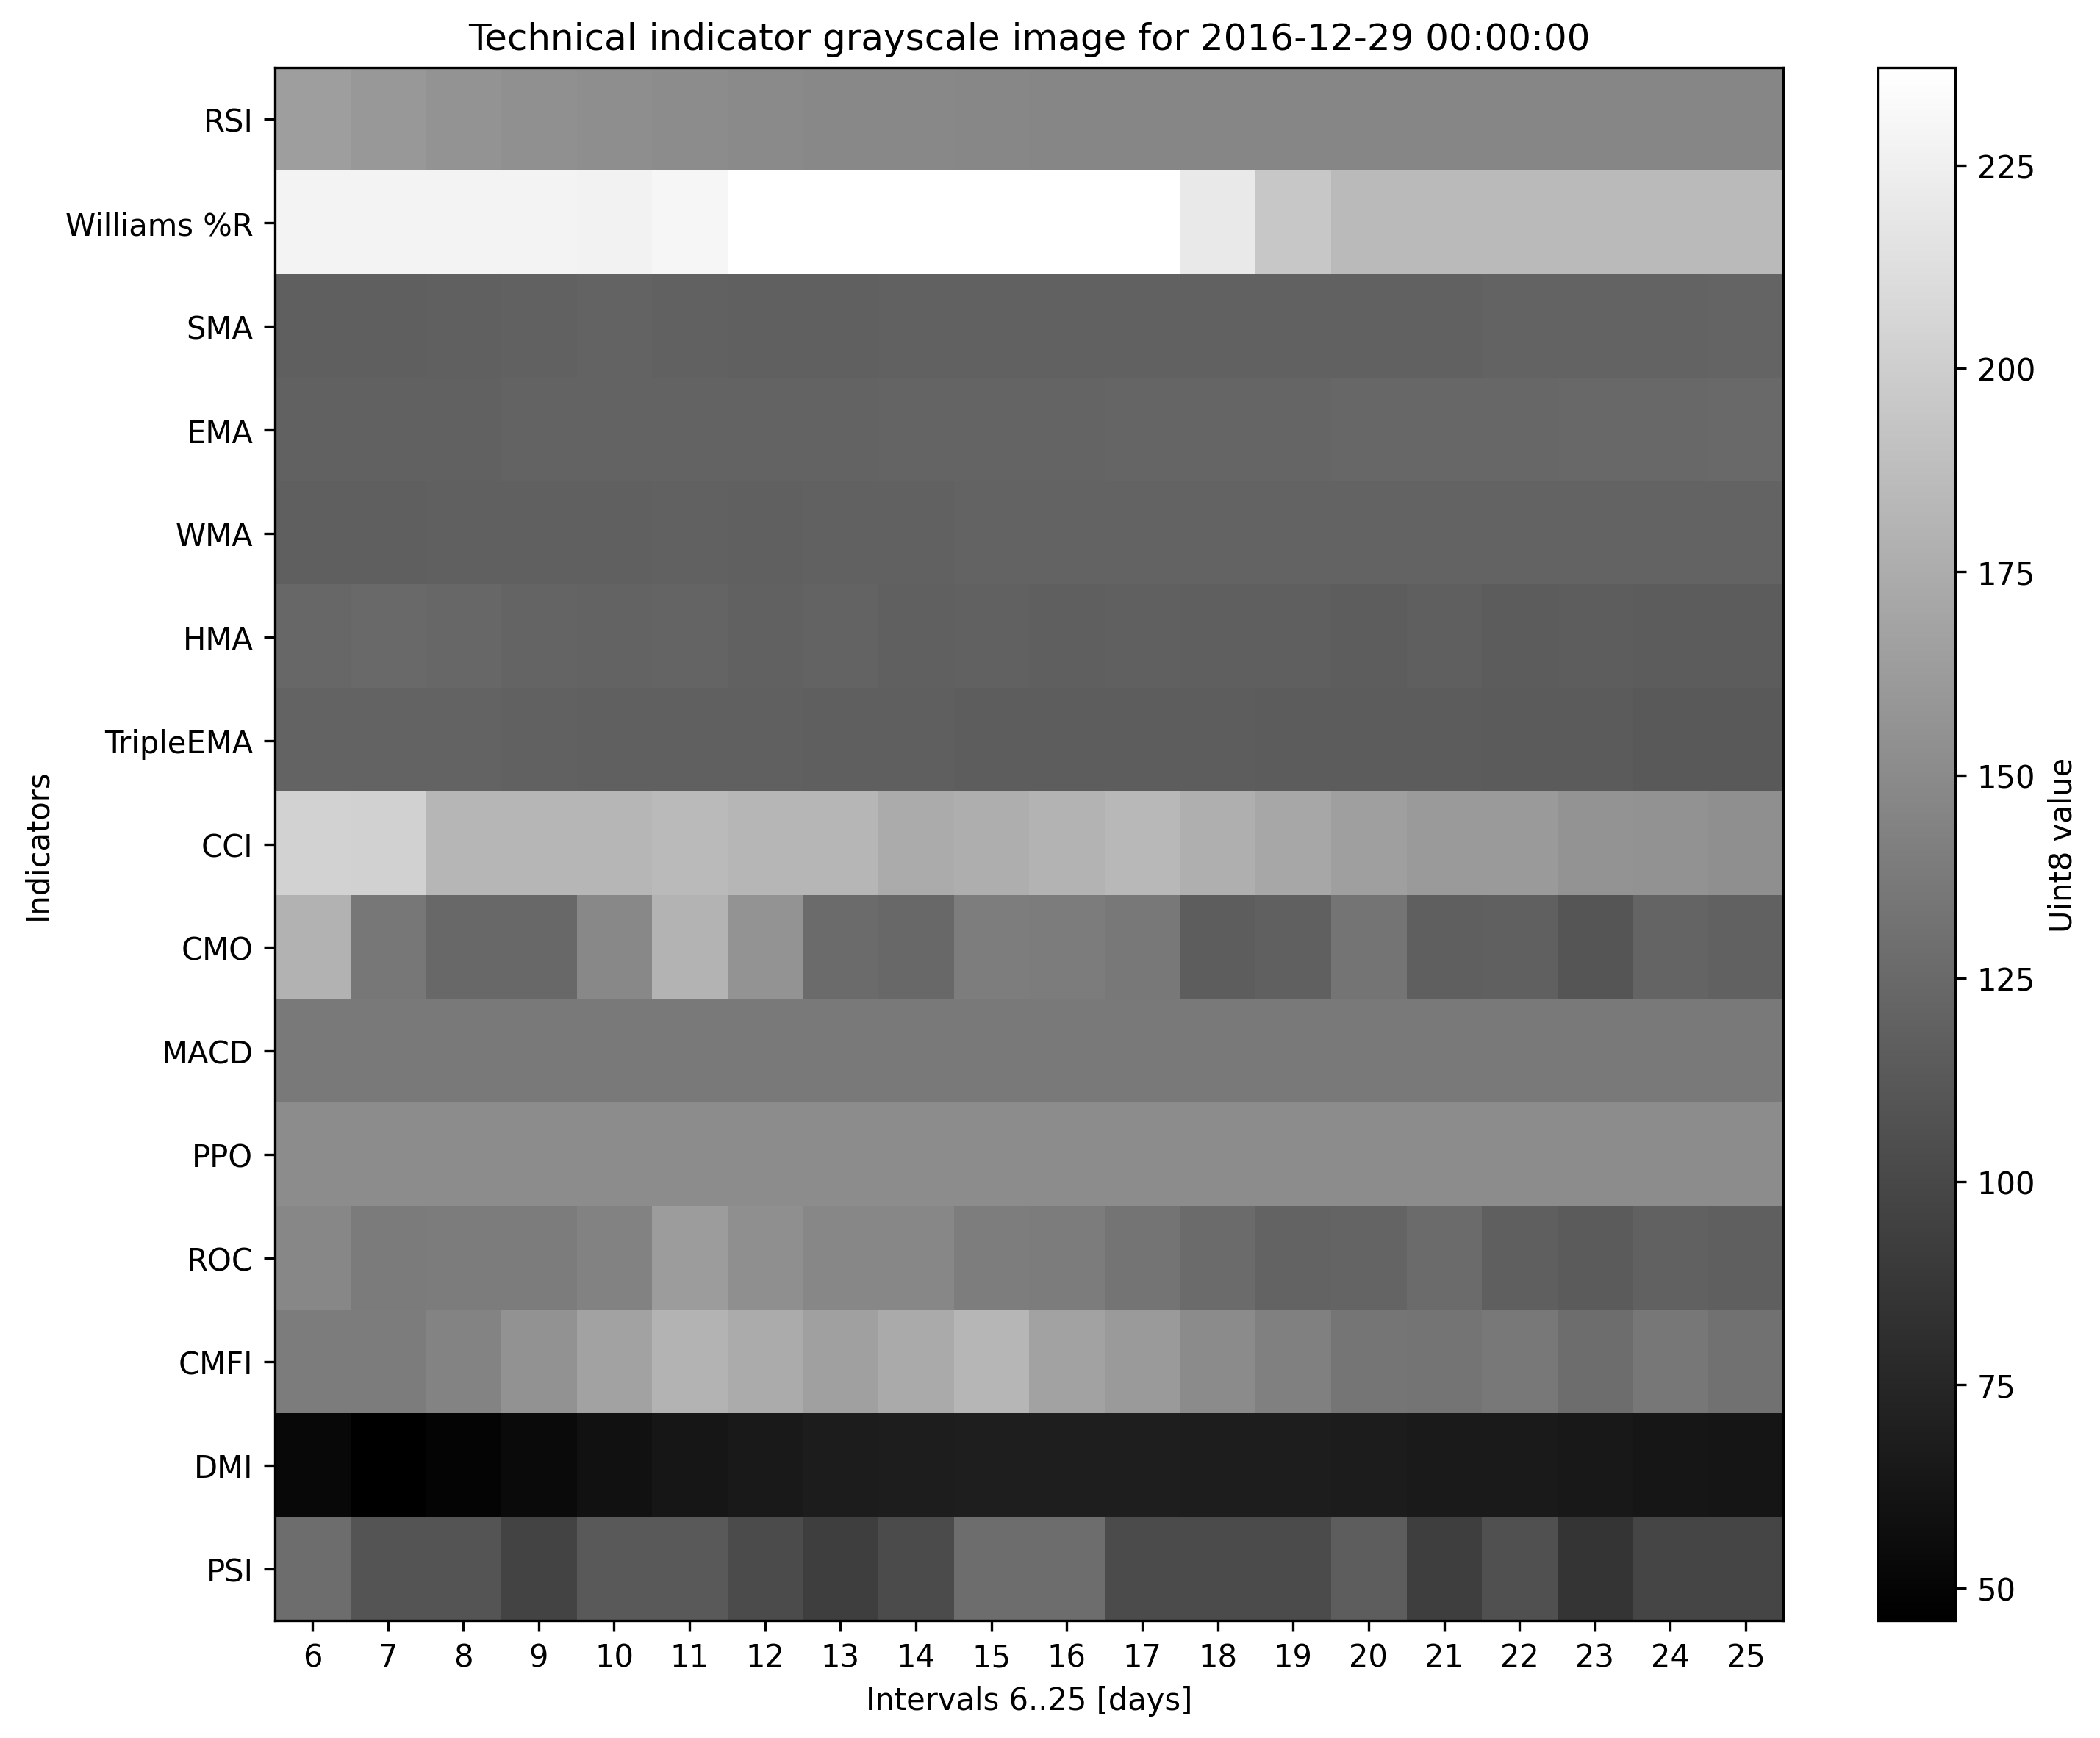
\includegraphics[width=0.85\textwidth]{../figures/Technical_Indicator.png}
	\caption{Example of a technical–only grayscale image ($15 \times 20$). The vertical axis shows the fifteen technical indicators, and the horizontal axis lists lookback windows from six to twenty–five days.}
	\label{fig:tech_only_image}
\end{figure}

Figure~\ref{fig:tech_macro_image} illustrates the combined representation, where the five macroeconomic rows are appended beneath the technical indicators to form a $20 \times 20$ image.


\begin{figure}[H]
	\centering
	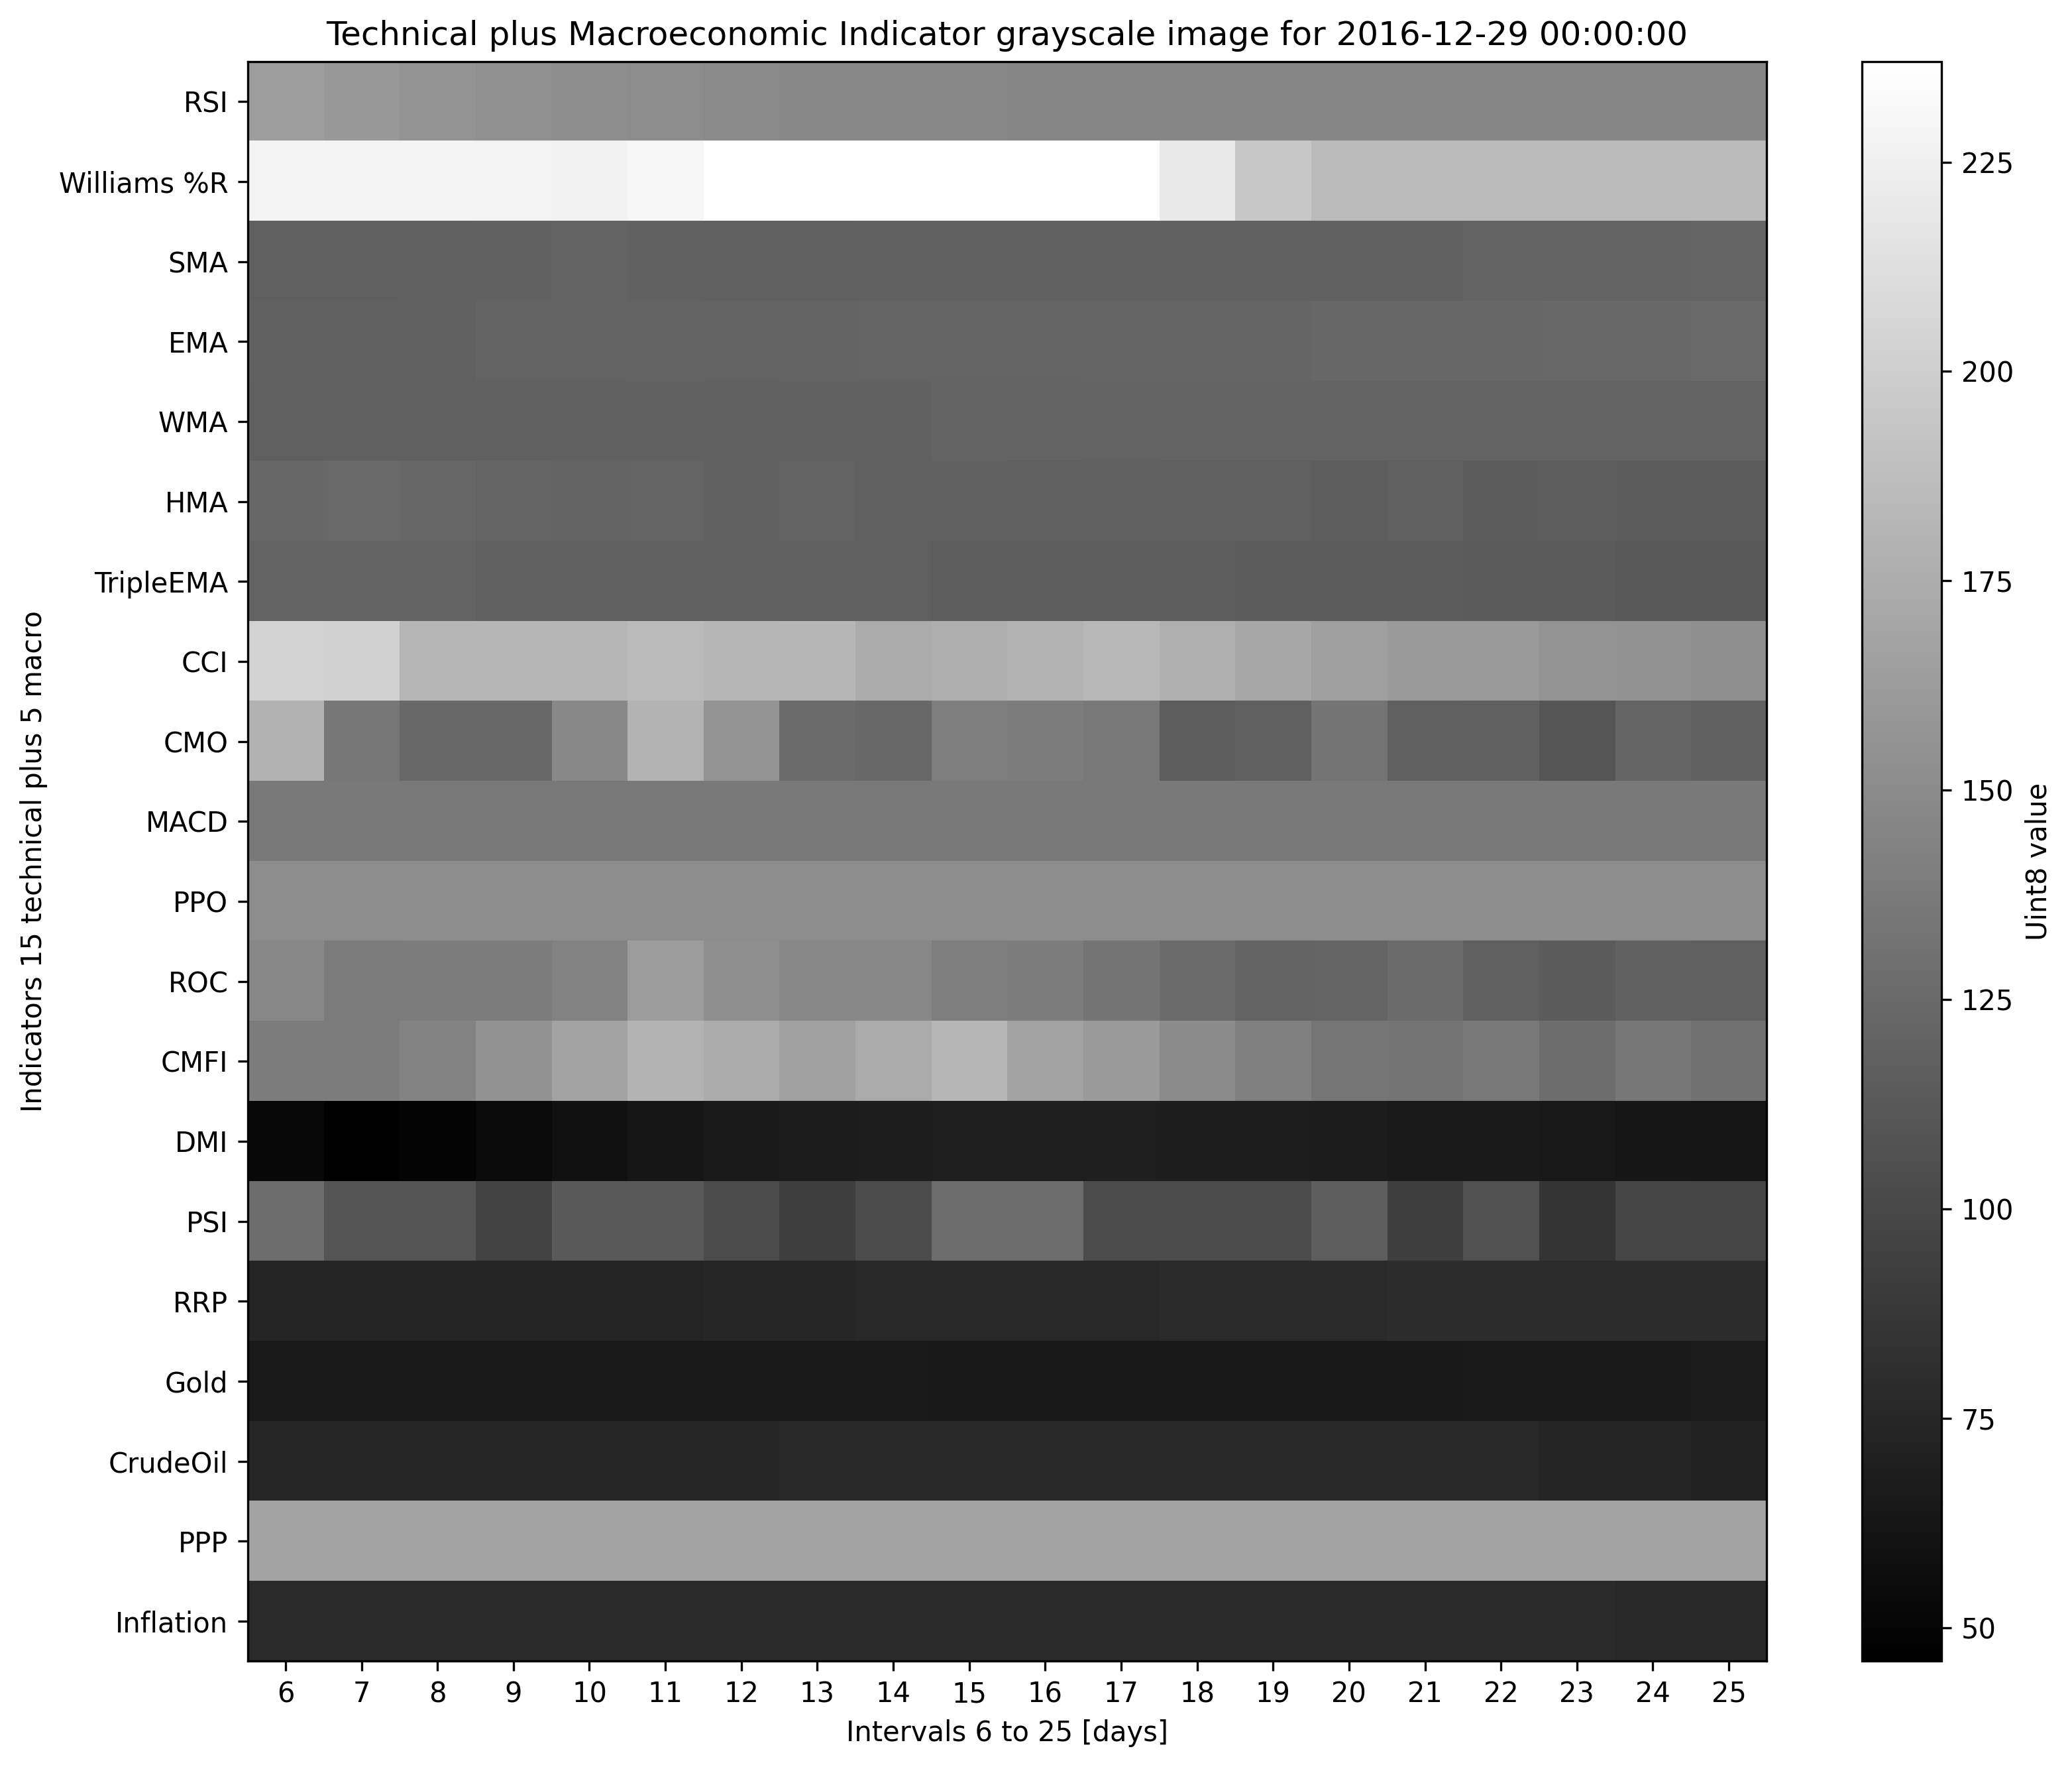
\includegraphics[width=0.85\textwidth]{../figures/CombinedTechandMacro.png}
	\caption{Combined technical and macroeconomic grayscale image ($20 \times 20$). Rows 16–20 contain RRP, Gold, CrudeOil, PPP, and Inflation, aligned to the same set of lookback windows.}
	\label{fig:tech_macro_image}
\end{figure}

In summary, the two representations show how normalized and quantized indicator values are translated into grayscale images. CNN--TIC uses a $15 \times 20$ technical-only image, while CNN--MIC uses a $20 \times 20$ image with additional macroeconomic context. These two image forms serve as input representations for the comparison of the baseline and proposed CNN models.

\subsection{Model Training}
\label{subsec:model-training}

This stage trains two convolutional models under identical settings to allow a fair comparison between the technical-only baseline and the combined technical–macroeconomic approach. The baseline model, CNN--TIC, receives a $15 \times 20$ grayscale image that encodes only the technical indicators. The proposed model, CNN--MIC, refers to a Convolutional Neural Network with Macroeconomic-Integrated Channels. It receives a $20 \times 20$ image where the technical indicators and the macroeconomic series are integrated into a single representation.


\begin{figure}[H]
	\centering
	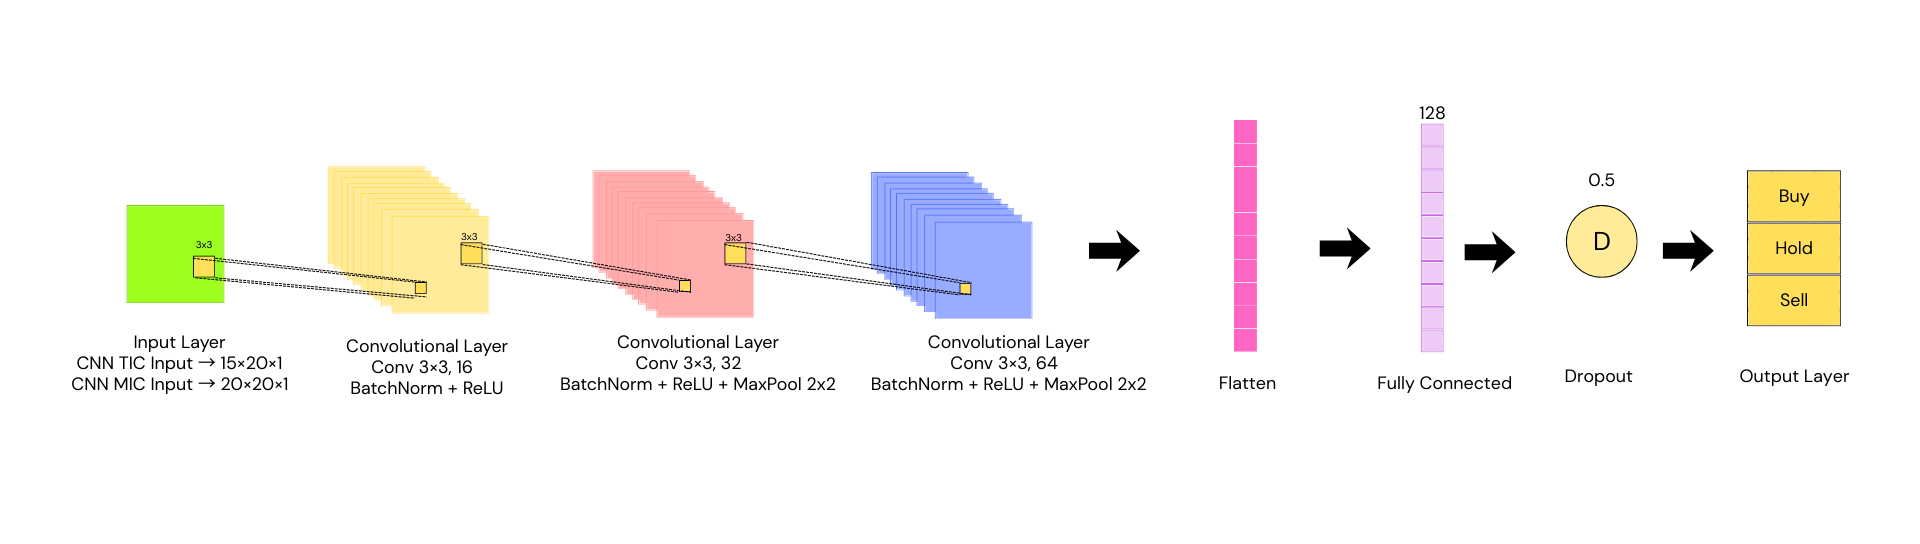
\includegraphics[width=1\textwidth]{../figures/CNN_Architecture.png}
	\caption{SmallCNN\_BN architecture used for both CNN--TIC and CNN--MIC. The network applies three convolutional blocks with batch normalization and ReLU, followed by flattening, a fully connected layer with 128 units, dropout, and a three-unit softmax output.}
	\label{fig:smallcnn-architecture}
\end{figure}

\paragraph{Architecture}

The architecture follows the design principles of earlier image-based trading systems such as CNN--TIC, which showed that shallow convolutional structures are effective for indicator-based images. In this study, the input images are much smaller than those used in standard vision applications. The technical-only images measure $15 \times 20$, and the combined images measure $20 \times 20$. Because of these constraints, deeper architectures and standard vision backbones are unsuitable.

To address this, a compact model called \textbf{SmallCNN\_BN} was constructed. The model adapts the general ideas demonstrated in prior CNN trading literature but is redesigned to match the spatial layout of the technical and macroeconomic representations. The objective is to provide enough capacity to detect local spatial patterns while controlling the risk of overfitting.

The feature extractor consists of three sequential convolutional blocks:

\begin{itemize}
	\item Block 1: Conv($3 \times 3$, 16 filters), BatchNorm, ReLU.
	\item Block 2: Conv($3 \times 3$, 32 filters), BatchNorm, ReLU, MaxPool($2 \times 2$).
	\item Block 3: Conv($3 \times 3$, 64 filters), BatchNorm, ReLU, MaxPool($2 \times 2$).
\end{itemize}

The output of the convolutional blocks is flattened and passed into a fully connected layer with 128 units and ReLU activation. A dropout layer (probability $0.5$) reduces overfitting. The final linear layer outputs three logits corresponding to the Buy, Hold, and Sell classes, followed by a softmax to produce class probabilities.

\paragraph{Training procedure}

Both models use the same training configuration to isolate the effect of the input representation. Weighted cross entropy is used as the loss function with a label smoothing factor of $0.05$. Class weights are computed from the training split using inverse class frequency to reduce the effect of strong class imbalance in the Buy and Sell categories.

Training uses the AdamW optimizer with a learning rate of $10^{-3}$, weight decay of $10^{-4}$, batch size of $128$, and a cosine annealing learning rate schedule. Each model is trained for $50$ epochs. For every cross-validation fold, the checkpoint with the highest validation macro F1 is retained.

\paragraph{Decision rule}

During inference, the predicted class for day $t$ is obtained by an argmax over the softmax probabilities:

\[
\hat{y}_t = \arg\max_{c \in \{\text{Buy, Hold, Sell}\}} \hat{p}_{t,c}.
\]

The class labels are then mapped into the trading actions used by the financial evaluation procedure described in Algorithm~\ref{alg:financial-evaluation}. This produces a sequence of actionable signals that are passed into the backtesting stage of the framework.

\begin{algorithm}[H]
	\footnotesize
	\caption{FinancialEvaluation}
	\label{alg:financial-evaluation}
	\begin{algorithmic}[1]
		\Procedure{FINANCIALEVALUATION}{}
		\State $balance = 10000$ PHP
		\State $bought\_amount = 0$
		\State $commission = 50$ PHP
		\State $take\_profit = 10\%$
		\State $stop\_loss = 1\%$
		\ForAll{$(price, predicted\_action)$ in $testDataset$}
		\If{$bought\_amount \neq 0$}
		\If{$price > take\_profit\_price$}
		\State $balance = bought\_amount * take\_profit\_price - commission$
		\State $bought\_amount = 0$
		\EndIf
		\If{$price < stop\_loss\_price$}
		\State $balance = bought\_amount * stop\_loss\_price - commission$
		\State $bought\_amount = 0$
		\EndIf
		\EndIf
		\If{$predicted\_action == BUY$ and $balance \neq 0$}
		\State $bought\_amount = (balance - commission) / price$
		\State $balance = 0$
		\State $take\_profit\_price = price * (1.0 + take\_profit / 100)$
		\State $stop\_loss\_price = price * (1.0 - stop\_loss / 100)$
		\EndIf
		\If{$predicted\_action == SELL$ and $bought\_amount \neq 0$}
		\State $balance = bought\_amount * price - commission$
		\State $bought\_amount = 0$
		\EndIf
		\EndFor
		\State \Return $balance$
		\EndProcedure
	\end{algorithmic}
\end{algorithm}


\subsection{Model Evaluation}
\label{subsec:model-eval}

This stage evaluates the models along two dimensions: classification accuracy and trading performance. The first set of metrics measures how well the models predict the Buy, Hold, and Sell classes. The second set measures how these predictions translate into financial outcomes when executed under a fixed trading strategy.

\paragraph{Classification metrics}

Accuracy and macro F1 are used to assess classification performance. These metrics are computed for every fold during cross-validation and averaged to obtain a stable estimate of model behavior. After training on the full training pool, the same metrics are computed on the test period to evaluate generalization.


\paragraph{Trading metrics}

To assess economic relevance, the predicted labels are converted into trading actions using the rules defined in Algorithm~\ref{alg:financial-evaluation}. The evaluation uses fixed parameters for both models to ensure a fair comparison. A Buy signal opens a long position on the next market open. A Sell signal closes any existing position. A Hold signal maintains the current position. Each transaction includes a 50-peso commission. The strategy applies a take-profit threshold of 10 percent and a stop-loss threshold of 1 percent relative to the entry price.

\paragraph{Output}

The procedure produces yearly returns, mean annual return, and final equity for the test period. These metrics allow the framework to determine whether improvements in representation lead to measurable gains in trading performance under identical simulation settings.

